\documentclass[12pt,a4paper]{article}

% Packages
\usepackage{geometry}
\geometry{margin=1in}
\usepackage{fancyhdr}
\usepackage{titlesec}
\usepackage{listings}
\usepackage{xcolor}
\usepackage{graphicx}

% Header & Footer
\pagestyle{fancy}
\fancyhf{}
\rhead{DBT - Assignment 6}
\lhead{Kamithkar Vinod}
\cfoot{\thepage}

% Title formatting
\titleformat{\section}{\large\bfseries}{Problem \thesection:}{0.5em}{}
\titleformat{\subsection}[runin]{\bfseries}{Code:}{0.5em}{}[---]
\titleformat{\subsubsection}[runin]{\bfseries}{Output:}{0.5em}{}[---]

% SQL language definition for listings
\lstdefinelanguage{SQL}{
  morekeywords={
    SELECT, FROM, WHERE, GROUP, BY, ORDER, ASC, DESC, JOIN, ON, AS,
    AND, OR, NOT, IN, IS, NULL, LIKE, HAVING, COUNT, SUM, AVG, MIN, MAX,
    CREATE, TABLE, INSERT, INTO, VALUES, UPDATE, SET, DELETE, DISTINCT,
    CASE, WHEN, THEN, ELSE, END, BETWEEN, EXISTS, UNION, ALL, ANY, LEFT,
    RIGHT, INNER, OUTER, LIMIT, OFFSET, PROCEDURE, BEGIN, FUNCTION, END, RETURNS, RETURN
  },
  sensitive=false,
  morecomment=[l]{--},
  morestring=[b]',
}

\lstset{
    language=SQL,
    basicstyle=\ttfamily\small,
    keywordstyle=\color{blue}\bfseries,
    commentstyle=\color{gray}\itshape,
    stringstyle=\color{red},
    showstringspaces=false,
    frame=single,
    breaklines=true,
    numbers=none
}

% Document Start
\begin{document}

% Title Page
\begin{center}
    \LARGE \textbf{Assignment - 6} \\[0.5cm]
    \Large \textbf{DBMS} \\[1cm]

    \begin{tabular}{rl}
        \textbf{Name:} & Kamithkar Vinod \\
        \textbf{Course:} & PG DAC AUGUST 2025 \\
        \textbf{PRN:} & 250850320040 \\
        \textbf{Form No:} & 250500480 \\
        \textbf{Date:} & 28-10-2025 \\
    \end{tabular}
\end{center}

\vspace{1cm}
\hrule
\vspace{0.5cm}

% Problems

% 1
\section{CURSOR}
\textbf{Task:} Update the total_amount in the orders table using the corresponding
product price from the products table.

\subsection{}
\begin{lstlisting}
DELIMITER //
CREATE PROCEDURE update_orders_total_amount()
BEGIN
    DECLARE done INT DEFAULT 0;
    DECLARE oid INT;
    DECLARE pid INT;
    DECLARE qty INT;
    DECLARE pr DECIMAL(10,2);
    DECLARE cur CURSOR FOR SELECT order_id, product_id, quantity FROM orders;
    DECLARE EXIT HANDLER FOR NOT FOUND SET done = 1;

    OPEN cur;
    cur_loop: LOOP
        FETCH cur INTO oid, pid, qty;
        IF done THEN
            LEAVE cur_loop;
        END IF;
        SELECT price INTO pr FROM products WHERE product_id = pid;
        UPDATE orders SET total_amount = pr * qty WHERE order_id = oid;
    END LOOP;
    CLOSE cur;
END //
DELIMITER ;

CALL update_orders_total_amount();

\end{lstlisting}

\subsubsection{}
\begin{center}
    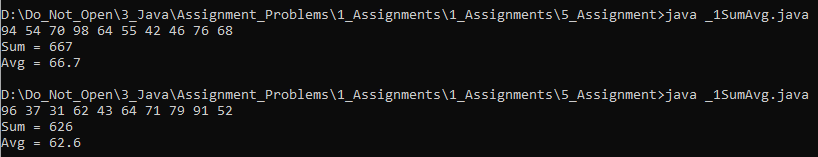
\includegraphics[width=0.8\textwidth]{1.png}
\end{center}

% 2

\section{CURSOR}
\textbf{Task:} Fetch all product names from the products table using a cursor and display them.

\subsection{}
\begin{lstlisting}
DELIMITER //
CREATE PROCEDURE fetch_product_names()
BEGIN
    DECLARE done INT DEFAULT 0;
    DECLARE pname VARCHAR(50);
    DECLARE cur CURSOR FOR SELECT product_name FROM products;
    DECLARE CONTINUE HANDLER FOR NOT FOUND SET done = 1;

    CREATE TEMPORARY TABLE names(name VARCHAR(50));

    OPEN cur;
    cur_loop: LOOP
        FETCH cur INTO pname;
        IF done THEN
            LEAVE cur_loop;
        END IF;
        INSERT INTO names VALUES (pname);
    END LOOP;
    CLOSE cur;

    SELECT * FROM names;
    DROP TEMPORARY TABLE IF EXISTS names;
END //
DELIMITER ;

CALL fetch_product_names();


\end{lstlisting}

\subsubsection{}
\begin{center}
    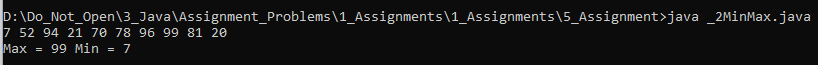
\includegraphics[width=0.8\textwidth]{2.png}
\end{center}

% 3

\section{CURSOR}
\textbf{Task:} Copy all data from the orders table into the order_audit table using a
cursor.

\subsection{}
\begin{lstlisting}
DELIMITER //
CREATE PROCEDURE copy_orders_to_audit()
BEGIN
    DECLARE done INT DEFAULT 0;
    DECLARE oid INT;
    DECLARE pid INT;
    DECLARE tamt DECIMAL(10,2);
    DECLARE cur CURSOR FOR SELECT order_id, product_id, total_amount FROM orders;
	DECLARE EXIT HANDLER FOR NOT FOUND SET done = 1;

    OPEN cur;
    loop1: LOOP
        FETCH cur INTO oid, pid, tamt;
        IF done THEN
            LEAVE loop1;
        END IF;
        INSERT INTO order_audit VALUES (oid, pid, tamt);
    END LOOP;
    CLOSE cur;
END //
DELIMITER ;

CALL copy_orders_to_audit();

select * from order_audit;

\end{lstlisting}

\subsubsection{}
\begin{center}
    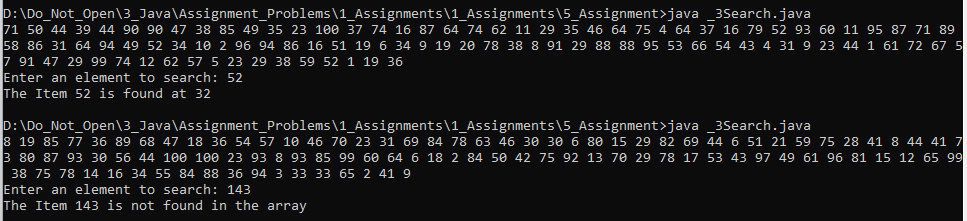
\includegraphics[width=0.8\textwidth]{3.png}
\end{center}

% 4

\section{CURSOR}
\textbf{Task:} Reduce the stock in the products table for each order processed according to the ordered quantity.

\subsection{}
\begin{lstlisting}
DELIMITER //
CREATE PROCEDURE reduce_stock_after_orders()
BEGIN
    DECLARE done INT DEFAULT 0;
    DECLARE pid INT;
    DECLARE qty INT;
    DECLARE cur CURSOR FOR SELECT product_id, quantity FROM orders;
    DECLARE EXIT HANDLER FOR NOT FOUND SET done = 1;

    OPEN cur;
    stock_loop: LOOP
        FETCH cur INTO pid, qty;
        IF done THEN
            LEAVE stock_loop;
        END IF;
        UPDATE products SET stock = stock - qty WHERE product_id = pid;
    END LOOP;
    CLOSE cur;
END //
DELIMITER ;

CALL reduce_stock_after_orders();

\end{lstlisting}

\subsubsection{}
\begin{center}
    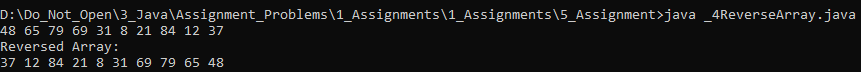
\includegraphics[width=0.8\textwidth]{4.png}
\end{center}

% 5

\section{CURSOR}
\textbf{Task:} Display all product names that are out of stock using a cursor.

\subsection{}
\begin{lstlisting}
DELIMITER //
CREATE PROCEDURE display_out_of_stock()
BEGIN
    DECLARE done INT DEFAULT 0;
    DECLARE pname VARCHAR(50);
    DECLARE cur CURSOR FOR SELECT product_name FROM products WHERE stock <= 0;
    DECLARE CONTINUE HANDLER FOR NOT FOUND SET done = 1;

    OPEN cur;
    read_loop: LOOP
        FETCH cur INTO pname;
        IF done THEN
            LEAVE read_loop;
        END IF;
        SELECT CONCAT(pname, ' is out of stock') AS message;
    END LOOP;
    CLOSE cur;
END //
DELIMITER ;

CALL display_out_of_stock();

\end{lstlisting}

\subsubsection{}
\begin{center}
    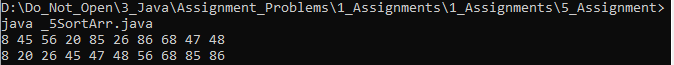
\includegraphics[width=0.8\textwidth]{5.png}
\end{center}

% 6

\section{CURSOR}
\textbf{Task:} Calculate and display the average price of all products using a cursor.

\subsection{}
\begin{lstlisting}
DELIMITER //
CREATE PROCEDURE avg_product_price()
BEGIN
    DECLARE done INT DEFAULT 0;
    DECLARE pr DECIMAL(10,2);
    DECLARE total DECIMAL(10,2) DEFAULT 0;
    DECLARE countp INT DEFAULT 0;
    DECLARE cur CURSOR FOR SELECT price FROM products;
    DECLARE CONTINUE HANDLER FOR NOT FOUND SET done = 1;

    OPEN cur;
    loop_prices: LOOP
        FETCH cur INTO pr;
        IF done THEN
            LEAVE loop_prices;
        END IF;
        SET total = total + pr;
        SET countp = countp + 1;
    END LOOP;
    CLOSE cur;

    SELECT total / countp AS 'Average Product Price';
END //
DELIMITER ;

CALL avg_product_price();

\end{lstlisting}

\subsubsection{}
\begin{center}
    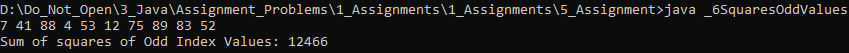
\includegraphics[width=0.8\textwidth]{6.png}
\end{center}

% 7

\section{CURSOR}
\textbf{Task:} Display all orders whose total amount is greater than ₹10,000 using a cursor.

\subsection{}
\begin{lstlisting}
DELIMITER //
CREATE PROCEDURE high_value_orders()
BEGIN
    DECLARE done INT DEFAULT 0;
    DECLARE oid INT;
    DECLARE amt DECIMAL(10,2);
    DECLARE cur CURSOR FOR SELECT order_id, total_amount FROM orders WHERE total_amount > 10000;
    DECLARE CONTINUE HANDLER FOR NOT FOUND SET done = 1;

    OPEN cur;
    hv_loop: LOOP
        FETCH cur INTO oid, amt;
        IF done THEN
            LEAVE hv_loop;
        END IF;
        SELECT CONCAT('Order ', oid, ' amount ₹', amt, ' is a high-value order') AS message;
    END LOOP;
    CLOSE cur;
END //
DELIMITER ;

CALL high_value_orders();

\end{lstlisting}

\subsubsection{}
\begin{center}
    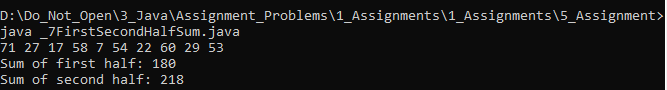
\includegraphics[width=0.8\textwidth]{7.png}
\end{center}

% 8

\section{CURSOR}
\textbf{Task:} Create a summary table showing each product and its total quantity sold using a cursor.

\subsection{}
\begin{lstlisting}
CREATE TABLE IF NOT EXISTS product_sales_summary (
    product_id INT,
    total_quantity INT
);

DELIMITER //
CREATE PROCEDURE create_sales_summary()
BEGIN
    DECLARE done INT DEFAULT 0;
    DECLARE pid INT;
    DECLARE qty INT;
    DECLARE cur CURSOR FOR SELECT product_id, quantity FROM orders;
    DECLARE EXIT HANDLER FOR NOT FOUND SET done = 1;

    TRUNCATE TABLE product_sales_summary;

    OPEN cur;
    sum_loop: LOOP
        FETCH cur INTO pid, qty;
        IF done THEN
            LEAVE sum_loop;
        END IF;
        INSERT INTO product_sales_summary(product_id, total_quantity)
        VALUES (pid, qty)
        ON DUPLICATE KEY UPDATE total_quantity = total_quantity + qty;
    END LOOP;
    CLOSE cur;
END //
DELIMITER ;

CALL create_sales_summary();
SELECT * FROM product_sales_summary;

\end{lstlisting}

\subsubsection{}
\begin{center}
    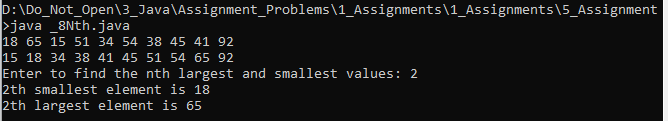
\includegraphics[width=0.8\textwidth]{8.png}
\end{center}

% 9

\section{CURSOR}
\textbf{Task:} Increase the price of all products with stock less than 5 by 10% using a cursor.

\subsection{}
\begin{lstlisting}
DELIMITER //
CREATE PROCEDURE increase_low_stock_price()
BEGIN
    DECLARE done INT DEFAULT 0;
    DECLARE pid INT;
    DECLARE pr DECIMAL(10,2);
    DECLARE cur CURSOR FOR SELECT product_id, price FROM products WHERE stock < 5;
    DECLARE EXIT HANDLER FOR NOT FOUND SET done = 1;

    OPEN cur;
    lp_loop: LOOP
        FETCH cur INTO pid, pr;
        IF done THEN
            LEAVE lp_loop;
        END IF;
        UPDATE products SET price = pr * 1.10 WHERE product_id = pid;
    END LOOP;
    CLOSE cur;
END //
DELIMITER ;

CALL increase_low_stock_price();

\end{lstlisting}

\subsubsection{}
\begin{center}
    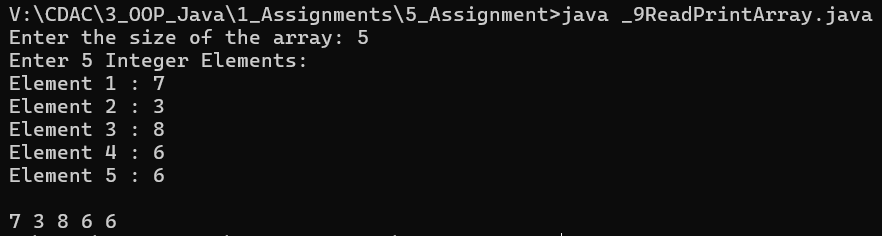
\includegraphics[width=0.8\textwidth]{9.png}
\end{center}

% 10

\section{CURSOR}
\textbf{Task:} Display all orders along with their corresponding product names and quantities
using a cursor.

\subsection{}
\begin{lstlisting}
DELIMITER //
CREATE PROCEDURE show_orders_with_product_names()
BEGIN
    DECLARE done INT DEFAULT 0;
    DECLARE oid INT;
    DECLARE pname VARCHAR(50);
    DECLARE qty INT;
    DECLARE cur CURSOR FOR
        SELECT o.order_id, p.product_name, o.quantity
        FROM orders o JOIN products p ON o.product_id = p.product_id;
    DECLARE CONTINUE HANDLER FOR NOT FOUND SET done = 1;

    OPEN cur;
    read_loop: LOOP
        FETCH cur INTO oid, pname, qty;
        IF done THEN
            LEAVE read_loop;
        END IF;
        SELECT CONCAT('Order ', oid, ': ', qty, ' x ', pname) AS details;
    END LOOP;
    CLOSE cur;
END //
DELIMITER ;

CALL show_orders_with_product_names();

\end{lstlisting}

\subsubsection{}
\begin{center}
    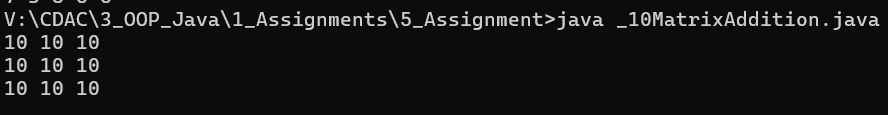
\includegraphics[width=0.8\textwidth]{10.png}
\end{center}



\end{document}
